\documentclass{beamer}

\usepackage{predavanja}
\usepackage{amsfonts}
\usepackage{array}
\usepackage{tikz}
\usetikzlibrary{intersections}

\newtheorem{izrek}{Izrek}

\title{Matematični izrazi in uporaba paketa \texttt{beamer}}
\subtitle{Vaje pri predmetu \emph{Računalniški praktikum}}
\institute{Fakulteta za matematiko in fiziko}
\date{}

\begin{document}

\begin{frame}
    \titlepage
\end{frame}

\begin{frame}{Kratek pregled}
    \tableofcontents[pausesections]
\end{frame}

\section{Paket \texttt{beamer}}
\begin{frame}{Posebnosti prosojnic}
    Za prosojnice je značilna uporaba okolja \texttt{frame}, s katerim
    definiramo posamezno prosojnico, postopno odkrivanje prosojnic,
    \pause
    ter nekateri drugi ukazi, ki jih najdemo v paketu \texttt{beamer}.
    \pause

    \begin{exampleblock}{Primer}
        Verjetno ste že opazili, da za naslovno prosojnico niste uporabili
        ukaza \texttt{maketitle}, ampak ukaz \texttt{titlepage}.
    \end{exampleblock}
\end{frame}

\begin{frame}{Poudarjeni bloki}
    \begin{block}{Opomba}
        Okolja za poudarjene bloke so \texttt{block},
        \texttt{exampleblock} in \texttt{alertblock}.
    \end{block}

    \begin{alertblock}{Opozorilo}
        Začetek poudarjenega bloka (ukaz \texttt{begin}) vedno sprejme
        dva argumenta: okolje in naslov bloka.

        Drugi argument (za naslov) je lahko prazen.
    \end{alertblock}
\end{frame}

\begin{frame}{Tudi v predstavitvah lahko pišemo izreke in dokaze}
    \begin{izrek}
        Praštevil je neskončno mnogo.
    \end{izrek}

    \begin{proof}
        Denimo, da je praštevil končno mnogo.

        \begin{itemize}[<+->]
            \item Naj bo \(p\) \alert<4>{največje} praštevilo.
            \item Naj bo \(q\) produkt števil \(1\), \(2\), \ldots, \(p\).
            \item Število \(q+1\) ni deljivo z nobenim praštevilom,
                  manjšim ali enakim \(p\).
            \item To je protislovje, saj ima \(q+1\)
                  praštevilskega delitelja, večjega od \(p\). \qedhere
        \end{itemize}
    \end{proof}
\end{frame}

\section{Paketa \texttt{amsmath} in \texttt{amsfonts}}
\begin{frame}{Postopno odkrivanje v okolju align}

Dokaži \emph{binomsko formulo}: za vsaki realni števili \(a\) in \(b\)
in vsako naravno število \(n\) velja
\begin{align*}
(a+b)^n \only<1>{&= \ldots \\}
\onslide<2->
&= (a+b)(a+b)\cdots(a+b) \\
\onslide<3->
&= a^n + n a^{n-1}b + \ldots + \binom{n}{k}a^{n-k}b^k + \ldots +
nab^{n-1} + b^n \\
&= \sum_{k=0}^{n} \binom{n}{k}a^{n-k}b^k
\end{align*}

\end{frame}

\section{Stolpci in slike}
\begin{frame}{Konstrukcija pravokotnice}
\begin{columns}[T,onlytextwidth]

\begin{column}{0.55\textwidth}
\small
\begin{itemize}
    \item<1-> Dana sta premica \(p\) in točka \(T\).
    \item<2-> Nariši lok \(l_1\) s središčem v \(T\).
    \item<3-> Lok \(l_1\) seka premico \(p\) v točkah \(A\) in \(B\).
    \item<4-> Nariši lok \(l_2\) s središčem v \(A\).
    \item<5-> Nariši lok \(l_3\) s središčem v \(B\) in z enakim polmerom.
    \item<6-> Loka se sečeta v točki \(C\).
    \item<7-> Premica \(TC\) je pravokotna na \(p\).
\end{itemize}
\end{column}

\begin{column}{0.45\textwidth}
\centering
\only<1>{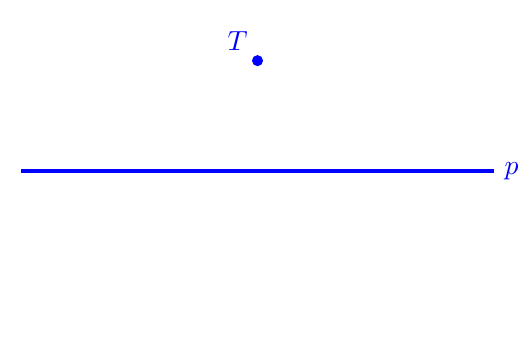
\includegraphics[width=\linewidth,keepaspectratio]{slike/fig-1.png}}
\only<2>{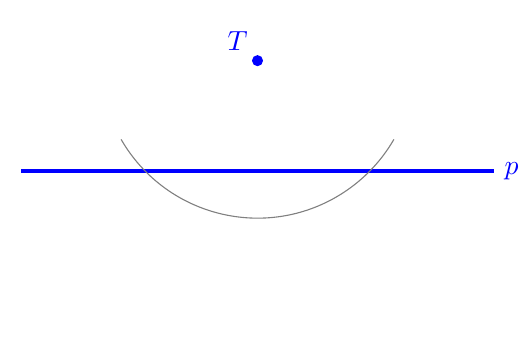
\includegraphics[width=\linewidth,keepaspectratio]{slike/fig-2.png}}
\only<3>{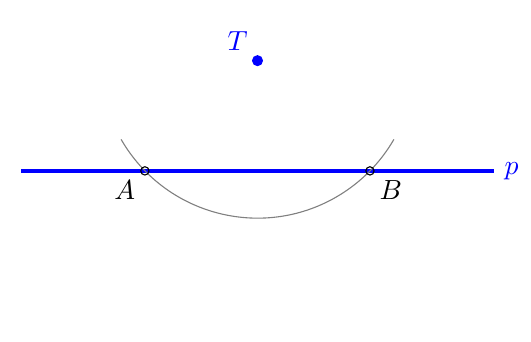
\includegraphics[width=\linewidth,keepaspectratio]{slike/fig-3.png}}
\only<4>{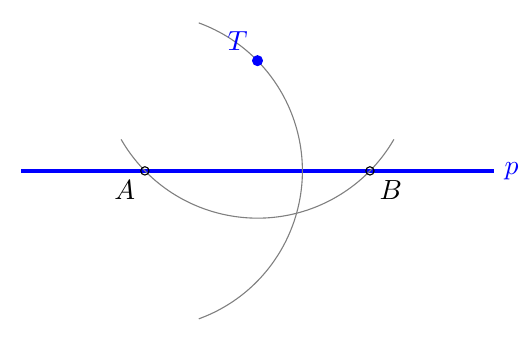
\includegraphics[width=\linewidth,keepaspectratio]{slike/fig-4.png}}
\only<5>{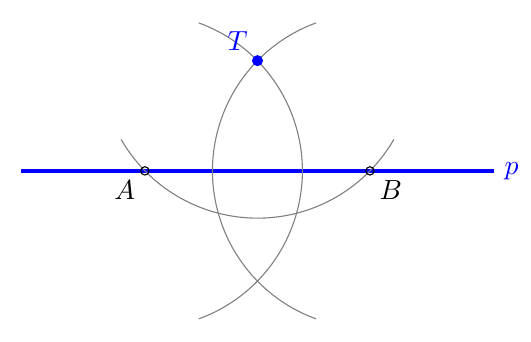
\includegraphics[width=\linewidth,keepaspectratio]{slike/fig-5.png}}
\only<6>{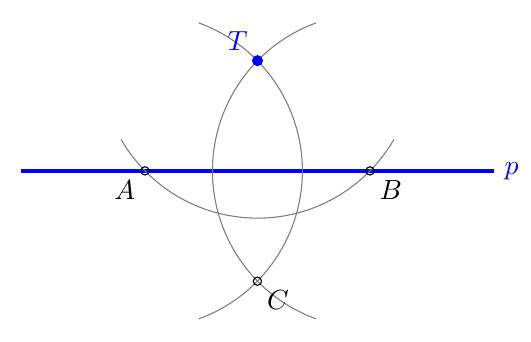
\includegraphics[width=\linewidth,keepaspectratio]{slike/fig-6.png}}
\only<7>{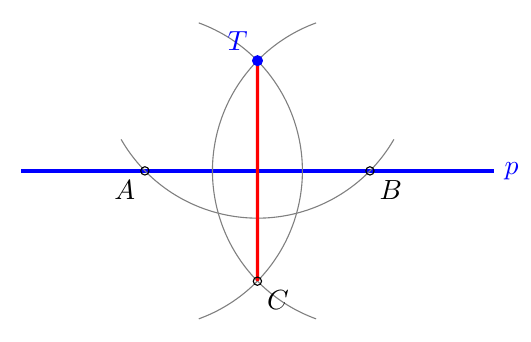
\includegraphics[width=\linewidth,keepaspectratio]{slike/fig-7.png}}
\end{column}

\end{columns}
\end{frame}

\section{Paket \texttt{beamer} in tabele}
\begin{frame}{Odkrivanje tabele po vrsticah}
    Včasih pride prav, da tabelo odkrivamo postopoma po vrsticah.

    \begin{center}
        \begin{tabular}{c|cccc}
            Oznaka & A & B & C & D \\ \hline
            \pause
            X & 1 & 2 & 3 & 4 \\
            \pause
            Y & 3 & 4 & 5 & 6 \\
            \pause
            Z & 5 & 6 & 7 & 8
        \end{tabular}
    \end{center}
\end{frame}

\begin{frame}{Odkrivanje tabele po stolpcih}
    Tabelo lahko odkrivamo tudi po stolpcih, čeprav ni najlažje.

    \begin{center}
        \begin{tabular}{c|>{\onslide<2->}c<{\onslide}>{\onslide<3->}c<{\onslide}>{\onslide<4->}c<{\onslide}>{\onslide<5->}c<{\onslide}}
            Oznaka & A & B & C & D \\ \hline
            X & 1 & 2 & 3 & 4 \\
            Y & 3 & 4 & 5 & 6 \\
            Z & 5 & 6 & 7 & 8
        \end{tabular}
    \end{center}
\end{frame}

\section{Risanje s paketom TikZ}
\begin{frame}{Konstrukcija pravokotnice}
    \centering
    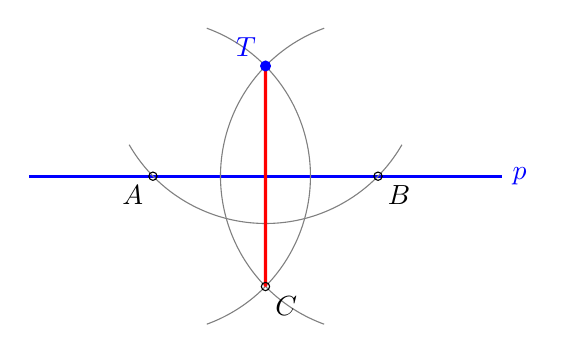
\begin{tikzpicture}
        \coordinate (T) at (0,1.4);

        \onslide<1->
        \draw[blue, very thick, name path=p] (-3,0) -- (3,0) node[right] {$p$};

        \onslide<2->
        \draw[gray, name path=k] (T) ++(210:2) arc (210:330:2);

        \onslide<3->
        \path[name intersections={of=p and k, by={A,B}}];

        \onslide<4->
        \draw[gray, name path=m] (A) ++(-70:2) arc (-70:70:2);

        \onslide<5->
        \draw[gray, name path=n] (B) ++(250:2) arc (250:110:2);

        \onslide<6->
        \path[name intersections={of=m and n, by={C,T'}}];

        \onslide<7->
        \draw[red, very thick] (T) -- (C);

        \onslide<1->
        \fill[blue] (T) circle (2pt) node[above left] {$T$};

        \onslide<3->
        \draw (A) circle (1.5pt) node[below left] {$A$};
        \draw (B) circle (1.5pt) node[below right] {$B$};

        \onslide<6->
        \draw (C) circle (1.5pt) node[below right] {$C$};
    \end{tikzpicture}
\end{frame}

\end{document}